\documentclass[../main.tex]{subfiles}
\graphicspath{{\subfix{../figures/}}}

\begin{document}
\section{实验原理}
\subsection{无线网络通信原理}
\subsubsection*{何为无线网络}
这里主要讲的是狭义上的无线网络, 即基于 802.11b/g/n 等标准的
\texttt{无线局域网(Wireless Local Area Network, WLAN)},
由于其具有可移动性、简单性、灵活性和高扩展能力, 作为对传统有线网络的延伸,
在许多特殊环境中得到了广泛应用.

IEEE 802.11 第一版发布于 1997 年, 其中定义了\texttt{介质访问接入控制层(MAC 层)}
和\texttt{物理层}. 物理层定义了工作在 $ 2.4 $ GHz 的 ISM 频段上的两种无线
调频方式和一种红外传输的方式, 总数据传输速率设计为 $ 2 $ Mbit/s.
两个设备间的通信可以\texttt{自由直接(ad-hoc)}的方式进行, 也可以在\texttt{基站(Base Station, BS)}
或者\texttt{访问点(Access Point, AP)}的协调下进行.

1999 年加上了两个补充版本:
\begin{enumerate}
  \item 802.11a 定义了一个在 $ 5 $ GHz ISM 频段上的数据传输速率可达 $ 54 $
    Mbit/s 的物理层;
  \item 802.11b 定义了一个在 $ 2.4 $ GHz 的 ISM 频段上, 但数据传输速率高达
    $ 11 $ Mbit/s 的物理层.
\end{enumerate}
%
\subsubsection*{无线网络组成}
\textbf{两个实体}:
\begin{itemize}
  \item \texttt{站点(Station)}: 通常指无线客户端.
  \item \texttt{接入点(Access Point)}: 无线接入点既有普通有线接入点的
    能力, 又有接入到上一层网络的能力. 从广义上讲, AP 就是无线路由器.
\end{itemize}

\textbf{两个服务单元}:
\begin{itemize}
  \item \texttt{基本服务单元(Basic Service Set, BSS)}: 网络最基本的服务单元,
    最简单的服务单元可以只由两个无线客户端组成, 就好比对等网. 客户端可以动态地
    连接(Associate)到基本服务单元中.
  \item \texttt{扩展服务单元(Extended Service Set, ESS)}:
    由分配系统和基本服务单元组合而成. 这种组合是逻辑上的.
    能力, 又有接入到上一层网络的能力. 从广义上讲, AP 就是无线路由器.
\end{itemize}
%
\subsubsection*{无线网络运作原理}
无线网络的设置至少需要一个 AP, 和一个或一个以上的无线 Client 即装有无线网卡的
客户端, 简称无线客户端. AP 每 $ 100 $ms 将 SSID(Service Set Identifier) 经由
Beacons(信号台)封包广播一次, Beacons 封包的长度相当短,
所以这个广播动作对网络效能的影响不大. 确保所有的 Wi-Fi Client 都能收到这个 SSID
的 AP 连接. 使用者可以设定要连接到哪个 SSID.

主要流程: 扫描(Scan) $ \rightarrow $ 认证(Authentication) $ \rightarrow $
关联(Association).

\begin{figure}[H]
  \begin{center}
    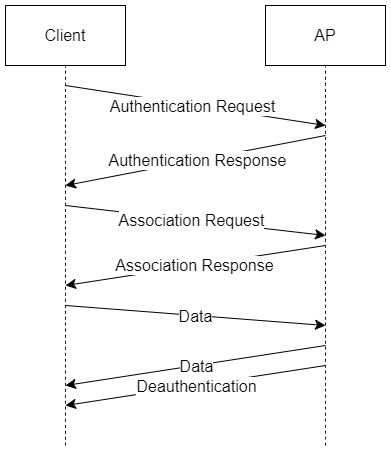
\includegraphics[width=0.20\textwidth]{wlan_communication.jpg}
  \end{center}
  \caption{无线网络运作原理}
\end{figure}
%
\subsection{Deauth Flood Attack}
Deauth 攻击是一种针对无线网络的常见攻击手段,
攻击者利用该攻击方式可以发送虚假的Deauthentication帧,
导致设备在接收到这些虚假帧后被迫断开与接入点的连接。
这种攻击行为使得受害者无法正常访问网络,频繁断网可能造成用户体验下降、
数据传输中断或网络服务不稳定等问题。

通过对Deauth攻击的实施,攻击者可以实现多种恶意行为,
包括但不限于对特定用户进行拒绝服务攻击、窃取用户网络通信数据、
诱导用户连接到恶意热点等,从而对网络安全和用户隐私构成威胁。

Deauth 攻击发生在 Wi-Fi 设备关联之后,其中引入了一个额外的实体,即攻击者(Attacker)。
攻击者可以通过执行 Deauth 攻击,迫使无线接入点(AP)下的任何一个用户频繁失去网络连接,
从而对其造成干扰。

\begin{figure}[H]
  \begin{center}
    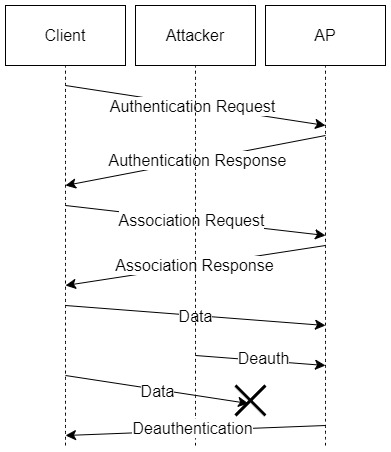
\includegraphics[width=0.20\textwidth]{deauth_flood_attack.jpg}
  \end{center}
  \caption{Deauth Flood Attack}
\end{figure}

在防御 Deauth 攻击方面,网络管理员可以采取一系列措施,
例如使用加密通信协议、监控网络流量、
限制无线网络访问权限等方式来加强网络安全,减少Deauth攻击的影响。
\end{document}
